% This file was created with tikzplotlib v0.10.1.
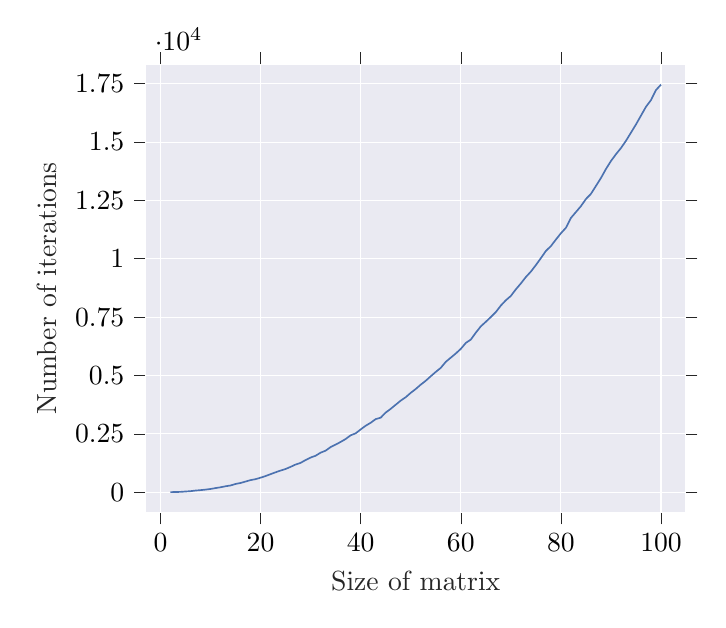
\begin{tikzpicture}

\definecolor{darkslategray38}{RGB}{38,38,38}
\definecolor{lavender234234242}{RGB}{234,234,242}
\definecolor{steelblue76114176}{RGB}{76,114,176}

\begin{axis}[
axis background/.style={fill=lavender234234242},
axis line style={white},
mark options={mark size=2.5pt, line width=1.5pt},
minor xtick={},
minor ytick={},
tick align=outside,
title style={align=center},
x grid style={white},
xlabel=\textcolor{darkslategray38}{Size of matrix},
xmajorgrids,
xmajorticks=false,
xmajorticks=true,
xmin=-2.9, xmax=104.9,
xtick style={color=darkslategray38},
xtick={-20,0,20,40,60,80,100,120},
y grid style={white},
ylabel=\textcolor{darkslategray38}{Number of iterations},
ymajorgrids,
ymajorticks=false,
ymajorticks=true,
ymin=-872.1, ymax=18336.1,
ytick style={color=darkslategray38},
ytick={-2500,0,2500,5000,7500,10000,12500,15000,17500,20000}
]
\addplot [semithick, steelblue76114176]
table {%
2 1
3 7
4 12
5 28
6 42
7 69
8 87
9 109
10 136
11 175
12 209
13 253
14 286
15 351
16 393
18 516
19 557
20 620
21 691
23 852
24 925
25 992
26 1084
27 1184
28 1255
29 1376
30 1484
31 1560
32 1693
33 1778
34 1932
35 2037
36 2152
37 2277
38 2436
39 2520
40 2687
41 2846
42 2973
43 3130
44 3192
45 3410
46 3570
48 3922
49 4068
50 4255
51 4419
52 4606
53 4773
54 4966
55 5152
56 5325
57 5584
59 5941
60 6138
61 6392
62 6536
63 6832
64 7104
65 7299
66 7502
67 7716
68 7995
69 8221
70 8407
71 8690
72 8942
73 9217
74 9449
75 9729
76 10026
77 10335
78 10542
79 10822
80 11092
81 11326
82 11748
84 12254
85 12560
86 12780
88 13460
89 13846
90 14188
91 14479
92 14744
93 15054
95 15756
97 16514
98 16798
99 17230
100 17463
};
\end{axis}

\end{tikzpicture}
